\documentclass{article}
\usepackage{amsmath,graphicx,verbatim,url,listings,fullpage,enumerate,csquotes}
%\usepackage[left]{lineno}
\begin{document}
%\linenumbers
%\title{Tool Setup for Deep Machine Learning}
\title{Designing Deep Learning Neural Networks using Caffe}
\author{Anurag Kishore\thanks{Currently Anurag is with Directi, Bangalore, India, Email: kishore.1337.anurag@gmail.com},~Stuti Jindal\thanks{Currently Stuti is with Cerner, Bangalore, India, Email: stuti.jindal11@gmail.com} and Sanjay Singh\thanks{Sanjay Singh is with the Department of Information \& Communication Technology, Manipal Institute of Technology, Manipal University, Manipal-576104, India}}

\maketitle

%\tableofcontents
\begin{abstract}
This tutorial investigates various tools for designing Deep Learning Neural Networks (DLNN). Our exploration of many tools has revealed that Caffe is the fastest and most appropriate tool for designing DLNNs. We have given step by step procedure for installing and configuring Caffe and its dependencies for designing DLNN. 
\end{abstract}
	
\section{Introduction}
Deep Learning is a field of Computer Science that involves use of deep networks for learning features from a dataset. Deep Neural Networks (DNN) are those neural networks that have more than one hidden layer. The number of hidden layers required to solve a problem has always been a topic of research in itself. Because most simple classification problems of low complexity require only one hidden layer, DNNs are often not targeted in regular Baccalaureate courses on Computer Science. However, a few recent developments in some fields have necessitated the use of deep neural networks, one of these fields is Computer Vision.
\par
Computer vision is a field that includes methods for acquiring, processing, analyzing, and understanding images and, in general, high-dimensional data from the real world in order to produce numerical or symbolic information \cite{ComputerVision:wiki}. Computer Vision may involve a learning based approach or an image processing approach with predefined features like object detection, object pose detection, video tracking, image restoration.
\par
This document focuses on Computer Vision using Machine Learning (AI) and discusses various tools and related strategies often required for the purpose of research and applications of this field.
\par
Rest of the report is organized as follows. First, we discuss the environment setup which involves an overview of multiple options available for Computer Vision via Machine Learning, followed by their evaluation and comparison. This section is intended to help people choose the environment which has most correlation with their purpose. Next, we discuss Caffe \cite{caffe} which is a framework for Deep Learning and we discuss specifics of setting it up. This is followed by an insight into its working and all that is required to get it to sing to your tunes.
\par
This document further provides a tutorial like approach to setting up Caffe on a machine learning testbed followed by a detailed discussion on its working and setting up of an example neural network. We have also discussed extending Caffe and/or editing layers to modify their behavior to fit the required solution.

\section{Learning Environments}
There are numerous Computer Vision libraries available to the average researcher. A list of the most notable ones are presented below:

\begin{itemize}
	\item OpenCV \cite{opencv}
	\item PyBrain \cite{pybrain}
	\item Theano \cite{theano}\cite{theano-scipy}
	\item MATLAB/R
	\item Weka \cite{weka}
	\item Caffe \cite{caffe}
\end{itemize}

\begin{enumerate}[a)]
	\item \textbf{OpenCV/C++} - A pure C++ implementation using the openCV library would require more time and effort in order to implement the basic infrastructure first. While this would definitely result in fast execution because of the native nature of C++ to most Operating Systems, this was not chosen for our research work because it would require time to merely reinvent the wheel.
	\item \textbf{PyBrain} - A Python Library designed for easy implementation of neural networks. It does not require the user to implement the basic infrastructure and allows the user to focus on the business logic instead. However, being a python implementation, it is slower than regular C++ implementation because of Python's nature.
	\item \textbf{Theano} - Theano is a Python library that allows efficient implementation of python code by converting the python code into C++. It also allows running the code on the GPU.
	\item \textbf{Matlab/R} - MATLAB and R are both languages designed for scientific and statistical applications. They have huge libraries each, allowing them to handle the menial tasks like implementation of basic infrastructure while the user focuses on the business logic. While both of the languages have libraries that can make the implementation easier, they are very slow during the execution phase and thus, using them is again, impractical as compared to the native implementations.
	\par	
MATLAB and R are both high level fourth generation programming language made for mathematical research. MATLAB is used widely in Electrical \& Electronic Circuit simulations, Control System simulations, Power System simulations, Machine Learning, Image Processing etc. R is a language made for statistical research purposes but it is more popular among Computer Science folk and is commonly used for machine learning, and sometimes preferred over MATLAB because it is a freeware whereas MATLAB is a proprietary tool.
	\item \textbf{Caffe} - It is a Deep Learning Framework introduced in \cite{caffe}, created by the Berkeley Vision and Learning Center (BVLC), UC Berkeley. It reduces the work of the user by allowing the user to define complex deep neural networks in a simple CSS-like language. However, internally, it uses the BLAS libraries, OpenCV library as well as nVidia's CUDA to generate highly optimized code in C++ with a possibility to use GPU to run it. It supports a variety of input types including raw image lists, LMDB, LevelDB, HDF5 multi dimensional data etc. Also, it provides a MATLAB library and a Python library for interfacing with other environments. The only drawback is that it only supports Linux, nevertheless there is an unofficial port for Windows, which has its own complications.
\end{enumerate}

\section{Caffe}
Caffe was chosen out of the above mentioned frameworks as well as over many other frameworks for our purposes because of the length of it's implementations, as well as due to the added bonus performance factor of OpenCV/BLAS/CUDA combination. It's major drawback, however, is the lack of a good GUI. There are also some issues regarding its setup process which need to be taken care of. This report illustrates step by step process for setting up Caffe for the required deep learning neural networks.

\section{Testbed Setup}
The recommended system requirement for setting up Caffe for the purpose of designing deep neural
network is given in Table 1.

\begin{table}[bpht!]
	\centering
	\caption{Recommended System Requirements}
	\begin{tabular}{|l|l|}
		\hline
		\textbf{Component} & \textbf{Configuration}\\
		\hline
		No. of processor cores & 4+ \\
		Processor clock frequency & 2.0+ GHz\\
		RAM & 16+GB\\
		GPU & nVidia Tesla\\
		Operating System & Latest version of a debian based linux (Ubuntu etc.) \\
		\hline
	\end{tabular}
\end{table}
It is preferable to have relatively higher system configuration in terms of parameters listed in Table 1 for the purpose of deep learning. Low-end systems might be able to install the framework but we noted that they would always fail at some point by running out of memory or segmentation faults. In some cases, this might even end up in an endless page-in, page-out cycle (Thrashing). On testbeds without GPUs, the iterations of the training process is very slow, thereby affecting productivity. A CPU with exceptional performance would be preferable if there is no GPU present on the system.
\par
The latest version of a debian based Linux is strongly recommended as it will halve the complexity of setting up Caffe on the system. In case a debian based Linux is not available on the testbed, any form of Linux should be preferred over Windows which should be preferred over other *nix based Operating Systems. This is because Linux architecture directly supported by the Caffe community and any issues will be resolved very quickly.

\section{Installation of Caffe}
An Internet connection is required for this installation procedure. In case the testbed is behind a proxy server, care needs to be taken to ensure that the testbed is properly configured with proxy server's details.
\par
A particularly tricky situation is when the proxy server is an authenticating server. In this case, it is recommended to install a secondary proxy software called CNTLM \cite{cntlm} which works both on windows and linux. Installation details of CNTLM may be found in Section 15 of this document.\\
\par
Presently Caffe is hosted at Berkeley's BVLC repository, which can be found at \url{https://github.com/BVLC/caffe}. The master branch of the repository is always the most stable build containing working code with proper unit tests. Caffe needs to be forked from this repository and then built on the target system. In order to do this, various other supporting libraries and software are required. They are mentioned as follows:-
\begin{itemize}
	\item nVidia CUDA
	\item OpenCV
	\item Boost
	\item BLAS Library
	\item GLOG - Google's Logging Library
	\item GFLAGS - Google's Flag Management Library
\end{itemize} 
\subsection{Ubuntu/Linux}
To use this git repository, one must have git installed on the testbed. The following code may be used to install git on the system:-
\begin{lstlisting}[tabsize=4,language=bash]
sudo apt-get install git #On ubuntu
sudo yum install git #On other linux
\end{lstlisting}

After git has been setup, a new command, '\texttt{git}' is now available. Use it to \enquote{pull} a repository's contents:
\begin{lstlisting}[tabsize=4,language=bash,breaklines]
cd /path/to/project/dir #Switch to parent of installation directory.
git clone https://github.com/BVLC/caffe caffe
\end{lstlisting}
This creates a local working copy of the repository in a directory called 'caffe'. Now, we need to make sure that all dependencies are resolved and all the support libraries that are required, are installed. This is done via:
\begin{lstlisting}[tabsize=4,language=bash,breaklines=true]
sudo apt-get install libprotobuf-dev libleveldb-dev libsnappy-dev libopencv-dev libboost-all-dev libhdf5-serial-dev libgflags-dev libatlas-base-dev python-devel libgoogle-glog-dev liblmdb-dev protobuf-compiler
\end{lstlisting}
In case the version of Ubuntu installation is less than 14.04, the last three libraries might cause issues during installation. In that case, the following commands, taken from \url{http://caffe.berkeleyvision.org/} might be required 
\begin{lstlisting}[tabsize=4,language=bash,breaklines]
# glog
wget https://google-glog.googlecode.com/files/glog-0.3.3.tar.gz
tar zxvf glog-0.3.3.tar.gz
cd glog-0.3.3
./configure
make && make install
# gflags
wget https://github.com/schuhschuh/gflags/archive/master.zip
unzip master.zip
cd gflags-master
mkdir build && cd build
export CXXFLAGS="-fPIC" && cmake .. && make VERBOSE=1
make && make install
# lmdb
git clone git://gitorious.org/mdb/mdb.git
cd mdb/libraries/liblmdb
make && make install
\end{lstlisting}

We also experimented with different versions of \emph{glog} and \emph{gflags}. The latest versions require an installation software called \emph{automake} to install. The latest versions of glog and gflags have issues working together and although it is possible to install them, it is much easier to use these versions as they are officially supported. After this is done, caffe may be installed on the system. Following steps guide to that goal. But before beginning, be sure to find out the path of all of the libraries stated above. They might be required.
\begin{lstlisting}[tabsize=4,language=bash,breaklines=true]
cd caffe 			#change to the caffe directory
cp Makefile.config.example Makefile.config #copy the Makefile example to the actual Makefile
\end{lstlisting}

Now, the makefile needs to be edited to add the Cuda path in its variable. All other libraries should work by default if their installation was successful as the example makefile is usually complete in itself. However, the includes directory list (\verb|INCLUDE_DIRS|) and the libraries directory list (\verb|LIBRARY_DIRS|) should be noted as further editing might be required in case the installation points out missing dependencies. After the editing of the makefile, enter the following commands in the caffe directory:
\begin{verbatim}
make all
make test
make runtest
\end{verbatim}

The 'make' command will automatically try to compile the files and link them while trying to resolve dependencies.
\subsubsection{Issues with Installation}
There might be various possible issues with installation. It is recommended to go to the official github repository of caffe and the caffe users Google group \cite{gg}. A few common issues that we faced are discussed below:

\begin{enumerate}[a)]
	\item \textbf{error: 'gflags' has not been declared}\\
	This happened to us because gflags had been installed with the namespace 'google'. In order to make it compatible with caffe, a snippet of code was placed in the various cpp files that raised the issue.
	\begin{lstlisting}[language=c++,breaklines]
	#ifndef GFLAGS_GFLAGS_H_
		namespace gflags = google;
	#endif
	\end{lstlisting}
	
	However, this line was not being executed, thus, we modified the first line to:
	\begin{lstlisting}[language=c++,breaklines]
	#ifdef GFLAGS_GFLAGS_H_
	\end{lstlisting}
	This was done, assuming that the macro was not defined. This was done in all of the five files that raised the issue. In one file, this code was not present, so we simply added the code at the beginning just after the include statements.
	
	\item textbf{Missing libraries}\\
	We also encountered some error messages like \texttt{libcudart.so was not found}. This means that the particular library is not in the directory specified in the \verb|LIBRARY_DIRS| variable. The solution is to simply find the libraries on the file system using the \verb|find| command in Linux and append the directory path to the \verb|LIBRARY_DIRS| variable.\\
	We had to add the atlas 64-bit library directory.
	\begin{lstlisting}[tabsize=4,language=bash,breaklines]
	/LIBRARY_DIRS := $(PYTHON_LIB) /usr/local/lib /usr/lib /usr/lib64/atlas$
	\end{lstlisting}
	
	\item textbf{Missing numpy headers}\\
	We also encountered a rather strange error that claimed that a few numpy headers were missing. We thus looked for them on our system and appended them to the \verb|PYTHON_INCLUDE| variable as follows:
	\begin{lstlisting}[tabsize=4,language=bash,breaklines]
	PYTHON_INCLUDE := /usr/include/python2.7 \
	/usr/local/include/python2.7 \
	/usr/lib/python2.7/dist-packages/numpy/core/include
	\end{lstlisting}
	Please note that the backslashes (\verb|\|) are used for separating multiline input.
\end{enumerate}

Apart from a few of these errors that we faced, the installation went fairly smooth on the Ubuntu and the RHEL testbed that we employed.

\subsection{Windows}
Windows is not directly supported by the Caffe community but there are ports of Caffe to Windows with cross compiled 64-bit libraries available. Niu Zhiheng's github repository \cite{nz} contains such cross compiled libraries along with a pre-configured, ready to install version of caffe along with the installation guide. His installation guide covers installation of caffe on a testbed having:
\begin{itemize}
	\item Windows 64-bit version
	\item Microsoft Visual Studio 2012
	\item CUDA Toolkit 6.5
\end{itemize}

In case a different version of caffe is being compiled, or the one from BVLC's repository is being compiled, Neil Shao's guide \cite{neil}, may be consulted. The guide is pretty concise with enough details and screenshots. However, there are no tutorials for building the python wrapper pycaffe on Windows using \texttt{cmake}. A MATLAB wrapper may be compiled in order to use caffe via MATLAB on windows, though. Otherwise, the best option available is to use the command line for using caffe.

\subsection{PyCaffe}
PyCaffe is the Python wrapper for Caffe which is placed inside the \verb|'python'| subdirectory of caffe. It may be built simply by running the following command:
\begin{lstlisting}[tabsize=4,language=bash,breaklines]
make pycaffe
\end{lstlisting}

PyCaffe's installation might require quite a few python libraries to be present. In case it points out that a few libraries are missing, they can be installed by running the following command:
\begin{lstlisting}[tabsize=4,language=bash,breaklines]
sudo pip install modulex #modulex is the name of the missing module.
sudo pip install --proxy=http://xx.yy.zz.ww:pp/ modulex #in case of proxy
\end{lstlisting}
Use the second command instead, in case of a proxy where \texttt{xx.yy.zz.ww:pp} is the proxy server's socket address.

\section{Caffe: Layer Catalogue}
The complete Caffe layer catalogue is available online at \cite{caffe:cl}. A few of the important layers are discussed below:
\begin{itemize}
	\item \textbf{Convolution Layer}\\
	Convolution Layer works on the principle of convolution which means applying a mathematical function to a range of values. This is most commonly used for abstracting images and other multidimensional input. An updated example based on the one from \cite{caffe:site} is presented below:
	\begin{lstlisting}[tabsize=2,breaklines=true]
	layer {
		name: "conv1"
		type: "Convolution"
		bottom: "input_blob_name" #Enter input blob name here.
		top: "output_blob_name"         # Enter output blob name here
		blobs_lr: 1          # learning rate multiplier for the filters
		blobs_lr: 2          # learning rate multiplier for the biases
		weight_decay: 1      # weight decay multiplier for the filters
		weight_decay: 0      # weight decay multiplier for the biases
		convolution_param {
			num_output: 96     # learn 96 filters
			kernel_size: 11    # each filter is 11x11
			stride: 4          # step 4 pixels between each filter
					# application
			weight_filler {
				type: "gaussian" # initialize the filters from a Gaussian
				std: 0.01        # distribution with stdev 0.01 
							# (default mean: 0)
			}
			bias_filler {
				type: "constant" # initialize the biases to zero (0)
				value: 0
			}
		}
	}
	\end{lstlisting}
	
	\item \textbf{Pooling Layer}\\
	A Pooling layer is a layer which works similar to a convolution layer but the function applied to the window is either the maximum value function (\verb|MAX|), the average value function (\verb|AVE|) or the stochastic function (\verb|STOCHASTIC|).
	\par	
	An example of a pooling layer is given below, an updated version of the example specified on \cite{caffe:site}:
	\begin{lstlisting}[tabsize=2,breaklines=true]
layer {
	name: "pool1"
	type: "Pooling"
	bottom: "input_blob"
	top: "output_blob"
	pooling_param {
		pool: MAX
	kernel_size: 3 # pool over a 3x3 region
	stride: 2   # step two pixels (in the 
						# bottom blob) between pooling regions
	}
}
	\end{lstlisting}
	
	\item \textbf{Dropout Layer}
	A fully connected layer is prone to overfitting. Nitish et al.,\cite{dropout} proposed a novel approach to avoid it. An example is given below:
	\begin{lstlisting}[tabsize=2,breaklines=true]
	layer { 
	name: "drop1" 
	type: "Dropout" 
	bottom: "target_blob" 
	top: "target_blob" 
	dropout_param { 
	dropout_ratio: 0.4 
	} 
	}
	\end{lstlisting}
	
	\item \textbf{Inner Product Layer}-the fully connected layer of caffe.
	\begin{lstlisting}[tabsize=2,breaklines=true]
	layer {
	name: "innerPrd"
	type: "InnerProduct"
	blobs_lr: 1          # learning rate multiplier for the filters
	blobs_lr: 2          # learning rate multiplier for the biases
	weight_decay: 1      # weight decay multiplier for the filters
	weight_decay: 0      # weight decay multiplier for the biases
	inner_product_param {
	num_output: 1000
	weight_filler {
	type: "gaussian"
	std: 0.01
	}
	bias_filler {
	type: "constant"
	value: 0
	}
	}
	bottom: "input_blob"
	top: "output_blob"
	}
	\end{lstlisting}
	\item \textbf{HDF5 Layers}
	HDF5 is a format which stores data in datasets which are $N$-dimensional arrays. So, virtually, any number of dimensions can be used to feed data to caffe. For example, for a batch of colour images, we use an HDF5 dataset of $batch\_size * channels * image\_width * image\_height$ dimensions. The HDF5 input layer takes in a text file containing a list of HDF5 files with maximum size of 2 GB each. The HDF5 output layer takes in the name of a non-existing file, in an existing directory, to which it saves two datasets containing one batch of 4D data and 2D labels containing the same number of instances. An example of the input layer is specified below:
	\begin{lstlisting}[tabsize=2,breaklines=true]
	layer {
	name: "hdf5in"
	type: "HDF5Input"
	input: "data"
	input: "label"
	hdf5_input_param {
	file_name: "/path/to/file.txt"
	}
	}
	\end{lstlisting}
	
	An example of the output layer follows:
	\begin{lstlisting}[tabsize=2,breaklines=true]
	layer {
	name: "hdf5out"
	type: "HDF5Output"
	bottom: "data"
	bottom: "label"
	hdf5_output_param {
	file_name: "dummy_output.h5"
	}
	}
	\end{lstlisting}
	
	We later discuss modification of the HDF5 output layer to expand it to store multiple batches of multiple outputs to datasets.
	
	\item \textbf{Memory Data Layer}\\
	Memory Data Layer is a layer designed for use with the python or MATLAB wrapper. It can directly point to data present already in the RAM in the form of variables etc. An example of Memory Data Layer follows:
	\begin{lstlisting}[tabsize=2,breaklines=true]
	layer {
	name: "data"
	type: "MemoryData"
	top: "data"
	top: "label"
	memory_data_param {  # blob dimensions
	batch_size: 60
	channels: 3
	height: 224
	width: 224
	}
	transform_param
	{
	crop_size: 256
	mirror: true
	mean_file: "path/to/meanfile.proto"
	}
	}
	\end{lstlisting}
	
	\item \textbf{Softmax Layer}
	A Softmax Layer, quite simply, generates a softmax distribution over all of the outputs. This is quite commonly used in multi-class classification to generate probabilities of the instance belonging to each class. An example is stated below:
	\begin{lstlisting}[tabsize=2,breaklines=true]
	layer { 
	name: "softmaxlayer" 
	type: "Softmax" 
	bottom: "prediction_output"
	top: "softmax_output"  
	} 
	\end{lstlisting}
\end{itemize}

\section{A Small Deep Network with Caffe}
Caffe uses Google's prototxt format for specification of neural networks. Each layer is defined separately and the inputs and outputs are multidimensional arrays called blobs. Layers are stacked vertically with the input at the bottom and the output at the top. Each layer expects a certain number of bottom and top blobs with certain dimensions. Chaining these blobs and layers results in a deep neural network.
\par
The following is a sample format of a layer in caffe having the type \verb|LayerType1|, having two input blobs and three output blobs:
\begin{lstlisting}[tabsize=2,breaklines=true]
layer {
name: "NameOfLayer"  # has to be unique
type: "LayerType1"  # has to be one of the types in layer catalogue
bottom: "bottom_blob_1"
bottom: "bottom_blob_2"
top: "top_blob_1"
top: "top_blob_2"
top: "top_blob_3"
layer_specific_params {
param1: value1
param2: "value2"
param3: value3
}
}
\end{lstlisting}

\begin{figure}[bpht!]
	\centering
	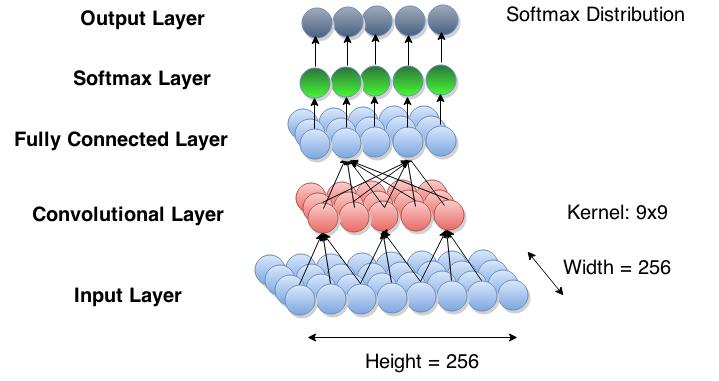
\includegraphics[scale=0.5]{Images/img_rating.jpg}
	\caption{A simple Deep Neural Network}
\end{figure}

Figure 1, shows a sample deep neural network. The normal structure of a deep neural network involves an input layer that takes input feature values, an output layer that computes the final prediction, a loss layer which might be integrated into the final output layer. The purpose of the loss layer is to compute the loss by comparing the labels to the predicted output in order to initiate backpropagation for weight updation.
\par
We will consider Fig.1 as the target for this tutorial. We will use this neural network to read images and their ratings (on a scale of one to five) for rating other images. The rating here, is merely the class id assigned to an image.
\par
Using caffe in the command line can be pretty disorienting for people used to GUIs at first, so proper organization of content is highly recommended. Create a directory called \verb|img_rating| inside the \verb|data| directory as well as the \verb|models| directory inside caffe's root directory. Create a file named \verb|img_rate.prototxt| in the \verb|models/img_rating| directory. Enter the following text in the prototxt file to name the network and then go on adding the subsequent layers as described.
\begin{lstlisting}[tabsize=2,breaklines=true]
name: "ImageRatingGenerator"
\end{lstlisting}

The first layer in the figure is the input layer. Caffe offers multiple input layers. For the purpose of this tutorial, ImageData Layer has been used. It takes an input text file which contains multiple lines of input. Each line contains an image file and the class id (an integer), separated as a space. It can also contain transformation parameters to modify the images read before sending them to the output blob. Two output blobs are generated. The first output blob contains a batch of the images and the second output blob contains a batch of the corresponding labels. Note that the layer only takes in integer labels. In case of multidimensional labels, use the HDF5 Input layer.
\begin{lstlisting}[tabsize=2,breaklines=true]
layer {
name: "Layer1"
type: "ImageData"
top: "data"
top: "label"
image_data_param {
file_name: "./data/img_rating/list.txt"
batch_size: 20
new_height: 256
new_width: 256
}
}
\end{lstlisting}

The second layer is a convolutional layer which has been explained already in the layer catalogue. Since this is an example, we will choose kernel\_size as nine with a stride of three and the number of outputs will be set to 100. These parameters depend on how deep the convolutional layer is placed in the network and what level of detail of features is being targeted.
\begin{lstlisting}[tabsize=2,breaklines=true]
layer {
name: "Layer2"
type: "Convolution"
bottom: "data"
top: "convolved_output"
blobs_lr: 1
blobs_lr: 2
weight_decay: 1
weight_decay: 0
convolution_param {
num_output: 100
kernel_size: 9
stride: 3
weight_filler {
type: "gaussian"
std: 0.01
}
bias_filler {
type: "constant"
value: 0
}
}
}
\end{lstlisting}

The third layer is a fully connected layer which generates a prediction on the classes possible. The number of outputs is equal to the number of classes.
\begin{lstlisting}[tabsize=2,breaklines=true]
layer {
name: "Layer3"
type: "InnerProduct"
bottom: "convolved_output"
top: "fc"
blobs_lr: 1
blobs_lr: 2
weight_decay: 1
weight_decay: 0
inner_product_param {
num_output: 5
weight_filler {
type: "gaussian"
std: 0.01
}
bias_filler {
type: "constant"
value: 0
}
}
}
\end{lstlisting}

The fourth layer is the Softmax Layer which generates a softmax distribution on the output of the fully connected layer. The softmax layer basically generates probabilities of the image belonging to each class.
\begin{lstlisting}[tabsize=2,breaklines=true]
layer {
name: "Layer4"
type: "SoftmaxWithLoss"
bottom: "fc"
top: "predict"
}
\end{lstlisting}
The fifth layer is the loss layer which computes the loss for backpropagation for training purposes. This can be included in the fourth layer by making it a SoftmaxWithLoss layer. This approach, however, will not return the output of the softmax layer as the top blob. Thus, for deploying the network, use the Softmax Layer instead.
\begin{lstlisting}[tabsize=2,breaklines=true]
layer {
name: "Layer4"
type: "SoftmaxWithLoss"
bottom: "fc"
bottom: "label"
top: "loss"
}
\end{lstlisting}

Now, your network is ready. To prepare the dataset, collect about 100 images and place them in the \verb|data/img_rating| directory. Create a text file with all the image names and label the images as well by rating the images on a scale of one to five with one being worst looking and five being best looking. We recommend the use of python to generate the list of images and then, opening the images in an image viewer and quickly appending each line with your rating, open in the alternate window. The following code snippet might help with that:
\begin{lstlisting}[language=Python,breaklines,showstringspaces=false]
import glob
# This will return a list of all files that
# match that wildcarded name string.
filelist = glob.glob('./data/img_rating/*.jpg')
# This will write it to a file.
filelist_file = open('./path/to/images/list.txt')
for filename in filelist:
filelist_file.write(filename)
filelist_file.close()
\end{lstlisting}

This will take care of the input data. Create another file named \verb|img_rating_solver.prototxt| and place it inside \verb|/models/img_rating|. Open it for editing and put the following text:
\begin{lstlisting}[tabsize=2,breaklines=true]
net: "models/img_rating/img_rate.prototxt" 
test_iter: 100
test_interval: 100
base_lr: 0.0001
lr_policy: "step" 
gamma: 0.1 
stepsize: 50
display: 20 
max_iter: 1000 
momentum: 0.9 
weight_decay: 0.0005 
snapshot: 20 
snapshot_prefix: "./models/img_rating/trained" # files will be saved with this prefix.
solver_mode: GPU
\end{lstlisting}

This solver learns by using the step learning procedure which is a form of learning rate annealing schedule \cite{Haykin:nn}. It basically slashes the learning rate down after each step of 50 iterations while using the momentum concept, for detail refer to \cite{Haykin:nn}). A snapshot of the trained weights is saved at every 20 iterations so that if the training stops due to any reason, it may be resumed from there. Execute this solver by running the command from the Caffe root directory:
\begin{lstlisting}[tabsize=4,language=bash,breaklines]
build/tools/caffe train --solver=./models/img_rating/img_rating_solver.prototxt --gpu=0
\end{lstlisting}

This will start the training procedure. As specified in the solver, the solving will stop after 1000 iterations. 

\section{Using the Python Interface}
The python interface to Caffe is called pycaffe. After compiling the pycaffe library, its location needs to be appended to the path to import it. It contains a wide variety of functions and wrappers to run caffe models. There are, currently, restrictions on which layers can be used with the python wrapper. Usage of layers which access files causes python to crash. Thus, for the input, usage of MemoryData Layer is recommended strongly if training of the network is required via Python. For training the network, the SGDSolver class of python is used but since training is already so easy via command line, in this section we will discuss classification via python wrapper. 
\par
Copy the previous tutorial's \verb|img_rate.prototxt| to the same folder, modifying the name to \verb|deploy_img_rate.prototxt|. And then, open the new file, remove the input layer from the file, and instead of it, add the following lines:
\begin{lstlisting}[tabsize=2,breaklines=true]
input: "data"
input_dim: 20
input_dim: 3
input_dim: 256
input_dim: 256
\end{lstlisting}
Also, revert the SoftmaxWithLoss Layer to Softmax layer as no loss layer is required and we need the output. Now, simply instantiate the network in ipython \cite{ipython}, load the image to be rated, and activate the network.

\begin{lstlisting}[language=Python,breaklines,showstringspaces=false]
import sys
sys.path.append('./python')  # Add the python 
# wrapper's path to sys.
import caffe                 # Previous statements 
# make this possible
MODEL_FILE = './models/img_rating/deploy_img_rating.prototxt'
PRETRAINED = './models/img_rating/trained_iter_1000.caffemodel'
IMAGE_FILE = './path/to/your/image/file/img.jpg'
net = caffe.Classifier(MODEL_FILE, PRETRAINED, image_dims=(256,256))
img = caffe.io.load_image(IMAGE_FILE)
pred = net.predict([img])    #Output of softmax layer.
print 'Rating: %d'%(pred[0].argmax())  #Display the output rating
\end{lstlisting}

\section{Working on Layers}
While Caffe's variety of layers is impressive, sometimes, one might need to extend the functionality of a layer, modify it, or simply, to find out its working. For instance, in our work, we required to know how was the loss being calculated in SoftmaxWithLoss layer and we also needed to modify the HDF5Output layer to allow saving of multiple blobs and batches. Caffe supports a multitude of layers which have been coded in C++ and CUDA for CPU as well as GPU implementations.
\par
For each layer in caffe, \verb|src/caffe/layers| contains a '.cpp' file and a '.cu' file. The CPP file contains two functions \verb|Forward_cpu()| and \verb|Backword_cpu()| whereas the CU file contains \verb|Forward_gpu()| and \verb|Backward_gpu()|. As the name suggests, these are the functions that contain code for the forward pass and backward pass of the CPU mode and the forward pass and backward pass of the GPU mode, respectively.
\par
For this tutorial, the problem of the HDF5Output layer will be discussed. The HDF5 layer works by taking in two blobs, \verb|data| and \verb|label| and saving their contents in one batch to the specified file as a dataset. It is, however, unable to save more than one batch at a time because HDF5 datasets should have unique names. Thus, we discuss a fix for this problem. This modification in the HDF5 Output layer alters the check in the \verb|include/caffe/data_layers.hpp| file to allow saving of multiple blobs to persistent storage.
\begin{lstlisting}[language=C++,breaklines]
//Comment this line out
/*virtual inline int ExactNumBottomBlobs() const { return 2; }*/  
virtual inline int MinBottomBlobs() const { return 1; }  //This line ensures multiple bottom blobs.
...
/*comment out the declaration of SaveBlobs and declare SaveBlob instead*/
//virtual void SaveBlobs();
virtual void SaveBlob(int, const vector<Blob<Dtype>*>&);
//Also add a variable to keep track of the current batch number:
int current_batch_;
\end{lstlisting}

Also, \verb|src/caffe/layers/hdf5_output_layer.cpp| is modified to include a new function called 'SaveBlob' which takes the blob number as well as the vector of bottom blobs to save the specified blob to disk as a dataset for the current batch. The \verb|Forward_cpu()| function just calls the \verb|SaveBlob()| function in a \texttt{for} loop. The constructor is also edited to initialize the new \verb|current_batch_| variable to zero. The variable is incremented once during each call to forward function.
\begin{lstlisting}[language=C++,breaklines]
template <typename Dtype> 
HDF5OutputLayer<Dtype>::HDF5OutputLayer(const LayerParameter& param) {
... // default code
current_batch_ = 0;
}
template HDF5OutputLayer<Dtype>::SaveBlob(int i, const vector<Blob<Dtype>*>& bottom) {
stringstream batch_id;
// Creating unique batch_id for the dataset.
batch_id << this->layer_param_.bottom(i) << "_" << current_batch_;
LOG_FIRST_N(INFO, bottom.size()) << "Saving batch " << batch_id.str() << " to file " << file_name_;
hdf5_save_nd_dataset(file_id_, batch_id.str(), *bottom[i]);
LOG(INFO) << "Saved";
}
template HDF5OutputLayer<Dtype>::Forward_cpu(const vector<Blob<Dtype>*>& bottom, const vector<Blob<Dtype>*>& top) {
CHECK_GE(bottom.size(), 1);  //Ensuring multiple blobs.
for(int i=0; i<bottom.size(), ++i){
SaveBlob(i, bottom);  // Saving each blob
}
H5Fflush(file_id_, H5F_SCOPE_GLOBAL);
current_batch_++;  //Incrementing batch number.
\end{lstlisting}

Now, after everything is done, just compile Caffe again with a \verb|make all| command and all should be working.

\section{Using HDF5 Layers}
The HDF5 Input layer requires the path of a text file which contains multiple lines of '.h5' files. The HDF5 layer produces all datasets as output blobs and thus, the number of top blobs and the number of datasets in the '.h5' file should match. The format is specified below:
\begin{lstlisting}[tabsize=2,breaklines=true]
layer {
name: "h5in"
type: "HDF5Data"
top: "data"
top: "label"
hdf5_data_param {
source: "path/to/files/list.txt"
batch_size: 30
}
}
\end{lstlisting}

The modified HDF5 output layer can be used to write predicted results to a file. This tutorial will try to classify the images from the earlier section of this tutorial and try to save the output ratings of images to a single file. In order to do this, add the following layer definitions at the end the \verb|models/img_rating/img_rate.prototxt|:
\begin{lstlisting}[tabsize=2,breaklines=true]
layer {
name: "Layer4Parallel"
type: "Softmax"
bottom: "fc"
top: "predict"
include { phase: TEST }
}
layer {
name: "h5in"
type: "HDF5Output"
bottom: "predict"
hdf5_data_param {
source: "path/to/files/list.txt"
}
include { phase: TEST }
}
\end{lstlisting}

These two layers are thus, added only during the \verb|TEST| state due to that include statement. However, now, it will generate multiple datasets in the same file, bearing different names. This can be run with a trained model by running the following command on the command line:

\begin{lstlisting}[tabsize=4,language=bash,breaklines]
./build/tools/caffe test --model=./models/img_rating/img_rate.prototxt --weights=./models/img_rating/trained_iter_1000.caffemodel --gpu=0
\end{lstlisting}

\section{Handling Authproxies via CNTLM}
CNTLM authentication proxy can be found at \cite{cntlm}. The windows version of CNTLM is an executable installer which easily installs CNTLM using a step by step wizard. On a linux machine, \texttt{apt-get} and \texttt{yum} might help:
\begin{lstlisting}[tabsize=4,language=bash]
sudo apt-get install cntlm #On ubuntu
sudo yum install cntlm #On other linux
\end{lstlisting}

If \texttt{apt-get} has problems with finding the package, a file named '\texttt{/etc/apt/sources.list}' should be checked to see if it has the universe repository enabled:
\begin{verbatim}
deb http://us.archive.ubuntu.com/ubuntu lucid main universe
\end{verbatim}

The update of \texttt{apt-get} followed by the above command should resolve problems on updated versions of Ubuntu. Configuration of the proxy server is the second step. It involves configuring CNTLM to act as a secondary proxy and tunnel data to the primary proxy. While the primary proxy uses authentication, we can make CNTLM not require authentication information, thus providing a no-authentication-required tunnel for data.
\par
After the installation is complete, CNTLM needs to be configured with the current proxy address and the username/domain combination. These may be found in the 'cntlm.ini' file on windows and the 'cntlm.conf' file in Linux. In these files, find the lines that begin with 'Username', 'Domain', 'Auth' and 'Proxy' and change them to:
\begin{verbatim}
Username		user1 #Where user1 is the name of the user
Domain			dom1 #Where domain1 is the name of the domain.
Auth			NTLMv2
...
Proxy			172.16.19.10:80 #Provide the proxy socket address here.
...
Listen			127.0.0.1:x #X is any port number. Preferably above 60,000.
\end{verbatim}

Now, open the command prompt or terminal and enter the following command:
\begin{lstlisting}
cntlm -c cntlm.ini -I -M http://caffe.berkeleyvision.org/ #For windows
cntlm -c cntlm.conf -I -M http://caffe.berkeleyvision.org/ #For Linux
\end{lstlisting}
This command tests the internet connection with the specified address and the configuration file. Then, it prompts the user for the proxy password and then returns an encrypted version of the password. Copy the information and paste it in the configuration file right after the 'Auth' field and the configuration is ready! Update all proxy address settings in the system and make sure it is running:
\begin{verbatim}
service cntlm start
\end{verbatim}

This should fix most of the proxy issues as sometimes, programs and libraries do not account for authenticating proxies.

\section*{Concluding Remarks}
This tutorial takes you through the step by step procedure for designing a deep learning neural network using Caffe.

\bibliographystyle{IEEEtran}
\bibliography{myref}
\end{document}